\documentclass[14pt]{beamer}

\mode<presentation>{ \usetheme{Madrid}

% To remove the navigation symbols from the bottom of all slides uncomment next line
\setbeamertemplate{navigation symbols}{}
\date{}
\title{}
\author{}

%to get rid of footer entirely uncomment next line
\setbeamertemplate{footline}{}
}

\usepackage{geometry}
\usepackage{multirow}
\usepackage{adjustbox}
\usepackage{multicol}
\setlength{\columnsep}{0.1cm}

\usepackage{tikz}
\usetikzlibrary{shapes, backgrounds}

\usepackage{bbding}
\usepackage{rotating}
\usepackage{xcolor}

%\usepackage{tkz-berge} %cool grid
\usepackage{pgfplots} %pics

\usepackage{graphicx} % Allows including images
\usepackage{
	booktabs
} % Allows the use of \toprule, \midrule and \bottomrule in tables
\usepackage{mathtools}

\newcommand{\R}{\mathbb{R}}
\newcommand{\Z}{\mathbb{Z}}
\newcommand{\N}{\mathbb{N}}
\newcommand{\e}{\varepsilon}

\newcommand{\p}{% \pause
}

% simple environrment for enumerate, easier to read
\setbeamertemplate{enumerate items}[default]

%%%%%%%%%%%%%%%%%%%%%%

% to use colours easily
\definecolor{miverde}{rgb}{0.7, .5, 0.7}
\newcommand{\azul}[1]{{\color{blue} #1}}
\newcommand{\rojo}[1]{{\color{red} #1}}
\newcommand{\verde}[1]{{\color{miverde} #1}}

% box in red and blue in math and outside of math
\newcommand{\cajar}[1]{\boxed{\mbox{\rojo{ #1}}}}
\newcommand{\majar}[1]{\boxed{\rojo{ #1}}}
\newcommand{\cajab}[1]{\boxed{\mbox{\azul{ #1}}}}
\newcommand{\majab}[1]{\boxed{\azul{ #1}}}

\newcommand{\setsize}[1]{\fontsize{#1}{#1}\selectfont} %allows you to change the font size. The default size of this document is 14. To change the font size of the whole slide, place this at the beginning of the slide. To change the size of only a portion of the text to size 12, you can do the following { \setsize{12} Your text. }.

\setbeamerfont{frametitle}{size=\fontsize{15}{15}\selectfont}
\setbeamerfont{block title}{size=\fontsize{14}{14}\selectfont}

\newcommand{\smallerfont}{\setsize{13}} %place this at the beginning of a slide to set the font size of the entire slide to 13.

%===========================

% For UNIT 2 specifically:

\newcommand{\floor}[1]{\lfloor #1 \rfloor}

%===================================================
\begin{document}
	%===================================================

	%-----------------------------

	%QUESTION_INFO: {"unit":2,"question":0,"title":"Properties of absolute value","images":[]}
	\begin{frame}
		\frametitle{Properties of absolute value}

		Let $a, b \in \mathbb{R}$. What can we conclude?

		\begin{enumerate}
			\item $\displaystyle |ab| = |a| |b|$

			\item $\displaystyle |a + b | = |a| + |b|$
		\end{enumerate}

		If any of the conclusions is wrong, fix it.
	\end{frame}

	%-----------------------------

	%QUESTION_INFO: {"unit":2,"question":1,"title":"Properties of inequalities","images":[]}
	\begin{frame}
		\frametitle{Properties of inequalities}

		Let $a, b, c \in \mathbb{R}$. \\ Assume $a < b$. What can we conclude?

		\begin{enumerate}
			\begin{multicols}{2}
				\item $\displaystyle a + c < b + c$

				\item $\displaystyle a- c < b - c$

				\item $\displaystyle ac < bc$

				\item $\displaystyle a^{2}< b^{2}$

				\item $\displaystyle \frac{1}{a}< \frac{1}{b}$
			\end{multicols}
		\end{enumerate}

		If any of the conclusions is wrong, fix it.
	\end{frame}

	%-----------------------------

	%QUESTION_INFO: {"unit":2,"question":2,"title":"Sets described by distance","images":[]}
	\begin{frame}
		\frametitle{Sets described by distance}

		Let $a \in \mathbb{R}$. Let $\delta >0$. \\ What are the following sets? Describe
		them using intervals

		\begin{enumerate}
			\item $\displaystyle A = \{x \in \mathbb{R}\; : \; |x| < \delta\}$

			\item $\displaystyle B = \{x \in \mathbb{R}\; : \; |x| > \delta\}$

			\item $\displaystyle C = \{x \in \mathbb{R}\; : \; |x-a| < \delta\}$

			\item $\displaystyle D = \{x \in \mathbb{R}\; : \; 0 < |x-a| < \delta\}$
		\end{enumerate}
	\end{frame}
	%-----------------------------

	%QUESTION_INFO: {"unit":2,"question":3,"title":"Implications","images":[]}
	\begin{frame}
		\frametitle{Implications}

		Find \emph{all} positive values of $A$, $B$, and $C$ which make the following
		implications true.

		\begin{enumerate}
			\item $\displaystyle | x-3 | < 1 \implies |2x-6| < A$

			\item $\displaystyle |x-3| < B \implies |2x-6| < 1$
			% \pause

			\item $\displaystyle |x-3| < 1 \implies |x+5| < C$
		\end{enumerate}
	\end{frame}
	%-----------------------------

	%QUESTION_INFO: {"unit":2,"question":4,"title":"Limits from a graph","images":["G1.svg","G1.png"]}
	\begin{frame}
		\frametitle{Limits from a graph}

		\begin{columns}[c]
			\column{.65\textwidth}

			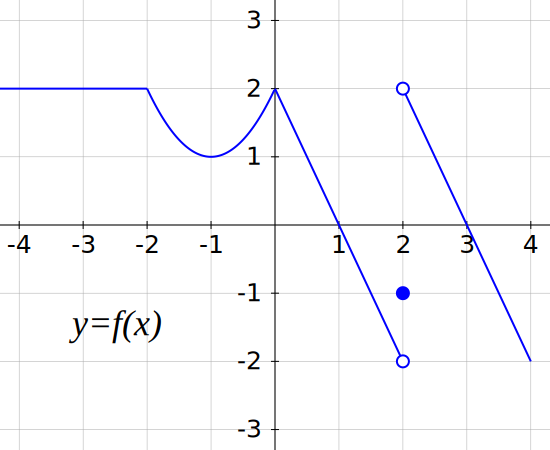
\includegraphics[scale=.4]{G1}

			\column{.33\textwidth}
			Find the value of
			\begin{enumerate}
				\item $\displaystyle \lim_{x \to 2}f(x)$

				\item $\displaystyle \lim_{x \to 0}f(f(x))$
				% \pause

				\item $\displaystyle \lim_{x \to 2}\left[ f(x) \right]^{2}$

				\item $\displaystyle \lim_{x \to 0}f(2 \cos x)$
			\end{enumerate}
		\end{columns}
	\end{frame}
	%-----------------------

	%QUESTION_INFO: {"unit":2,"question":5,"title":"Floor","images":[]}
	\begin{frame}[t]
		\frametitle{Floor}

		Given a real number $x$, we defined the \emph{floor of $x$}, denoted by $\lfloor
		x \rfloor$, as the largest integer smaller than or equal to $x$. For example:
		\[
			\lfloor \pi \rfloor= 3, \quad \quad \lfloor 7 \rfloor=7, \quad \quad \lfloor
			-0.5 \rfloor=-1.
		\]
		Sketch the graph of $\displaystyle y = \lfloor x \rfloor$. Then compute:
		\begin{multicols}{2}
			\begin{enumerate}
				\item $\displaystyle \lim_{x \to 0^+}\lfloor x \rfloor$

				\item $\displaystyle \lim_{x \to 0^-}\lfloor x \rfloor$

				\item $\displaystyle \lim_{x \to 0}\; \lfloor x \rfloor$

				\item $\displaystyle \lim_{x \to 0}\; \lfloor x^{2} \rfloor$
			\end{enumerate}
		\end{multicols}
	\end{frame}
	%-----------------------------

	%QUESTION_INFO: {"unit":2,"question":6,"title":"More limits from a graph","images":["G2.svg","G2.png"]}
	\begin{frame}
		\frametitle{More limits from a graph}

		\begin{columns}[c]
			\column{.65\textwidth}

			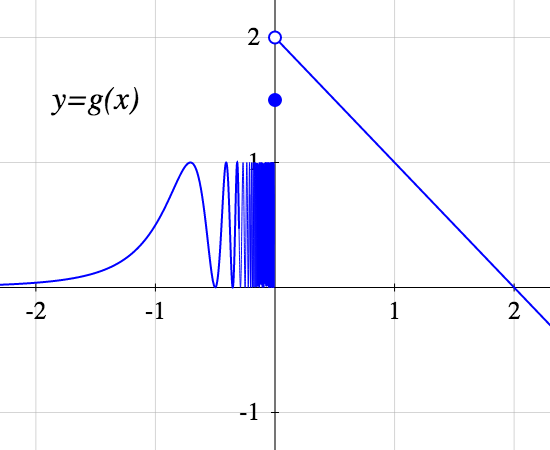
\includegraphics[scale=.4]{G2}

			\column{.33\textwidth}
			Find the value of
			\begin{enumerate}
				\item $\displaystyle \lim_{x \to 0^+}g(x)$

				\item $\displaystyle \lim_{x \to 0^+}\; \lfloor g(x) \rfloor$

				\item $\displaystyle \lim_{x \to 0^+}g(\lfloor x \rfloor)$

				\item $\displaystyle \lim_{x \to 0^-}g(x)$

				\item $\displaystyle \lim_{x \to 0^-}\; \lfloor g(x) \rfloor$

				\item $\displaystyle \lim_{x \to 0^-}\; \lfloor \frac{g(x)}{2}\rfloor$

				\item $\displaystyle \lim_{x \to 0^-}g(\lfloor x \rfloor)$
			\end{enumerate}
		\end{columns}
	\end{frame}

	%-----------------------------

	%QUESTION_INFO: {"unit":2,"question":7,"title":"Limit at a point","images":[]}
	\begin{frame}
		\frametitle{Limit at a point}

		If a function $f$ is not defined at $x=a$, then
		\begin{enumerate}
			\item $\displaystyle{\lim_{x\rightarrow a} f(x)}$ cannot exist

			\item $\displaystyle{\lim_{x\rightarrow a} f(x)}$ could be $0$

			\item $\displaystyle{\lim_{x\rightarrow a} f(x)}$ must approach $\infty$

			\item none of the above.
		\end{enumerate}
	\end{frame}

	%-----------------------------

	%QUESTION_INFO: {"unit":2,"question":8,"title":"Evaluating Limits","images":[]}
	\begin{frame}
		\frametitle{Evaluating Limits}

		\begin{itemize}
			\item You're trying to guess $\displaystyle{\lim_{x \rightarrow 0} f(x)}$.

			\item You plug in $x=0.1, 0.01, 0.001, \dots$ and get $f(x)=0$ for all these
				values.

			\item In fact, you're told that for all $n=1, 2, \dots$, $\displaystyle{f\left(\frac{1}{10^{n}}\right)}
				=0$. \\

			\item Can you conclude that $\displaystyle \lim_{x \rightarrow 0}f(x)=0$?
		\end{itemize}
	\end{frame}

	%-----------------------------

	%QUESTION_INFO: {"unit":2,"question":9,"title":"Exponential limits","images":[]}
	\begin{frame}
		\frametitle{Exponential limits}

		Compute:
		\[
			\lim_{t \to 0^+}e^{1/t}, \quad \quad \lim_{t \to 0^-}e^{1/t}.
		\]

		Suggestion: Sketch the graph of $\displaystyle y=e^{x}$ first.
	\end{frame}
	%------------------------------

	%QUESTION_INFO: {"unit":2,"question":10,"title":"Rational limits","images":[]}
	\begin{frame}[t]
		\frametitle{Rational limits}

		Consider the function
		\[
			h(x) = \frac{(x-1)(2+x)}{x^{2}(x-1)(2-x)}.
		\]
		\begin{itemize}
			\item Find all real values $a$ for which $h(a)$ is undefined. \\

			\item For each such value of $a$, compute
				$\displaystyle \lim_{x \to a^+}h(x)$ and
				$\displaystyle \lim_{x \to a^-}h(x)$. \\

			\item Based on your answer, and nothing else, try to sketch the graph of $h$.
		\end{itemize}
	\end{frame}
	%-----------------------------

	%QUESTION_INFO: {"unit":2,"question":11,"title":"$\\delta$ from a graph","images":["G3.svg","G3.png"]}
	\begin{frame}[t]
		\frametitle{$\delta$ from a graph}
		\fontsize{11}{11}\selectfont
		\begin{center}
			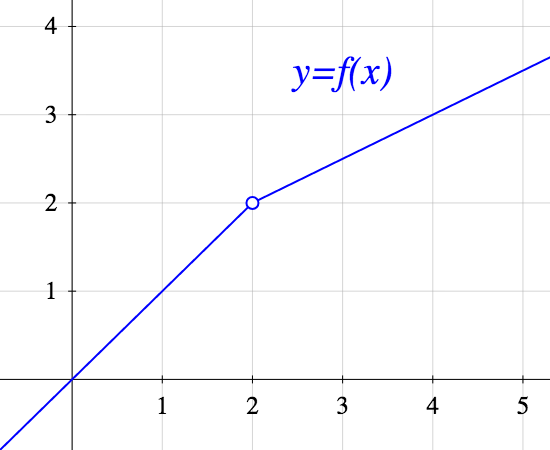
\includegraphics[scale=.3]{G3}
		\end{center}
		\begin{enumerate}
			\item Find one value of $\delta>0$ s.t. \hfill
				$\displaystyle 0 < |x-2| < \delta \implies |f(x) - 2| < 0.5$

			\item Find \emph{all} values of $\delta>0$ s.t. \hfill $\displaystyle 0 < |
				x-2| < \delta \implies |f(x) - 2| < 0.5$
		\end{enumerate}
	\end{frame}
	%-----------------------

	%QUESTION_INFO: {"unit":2,"question":12,"title":"Warm-up","images":[]}
	\begin{frame}
		\frametitle{Warm-up}

		Write down the formal definition of
		\[
			\lim_{x \to a}f(x) = L.
		\]
	\end{frame}

	%-----------------------------

	%QUESTION_INFO: {"unit":2,"question":13,"title":"Side limits","images":[]}
	\begin{frame}
		\frametitle{Side limits}

		\begin{block}{Recall}
			Let $L, a \in \mathbb{R}$. \\ Let $f$ be a function defined at least on an
			interval around $a$, except possibly at $a$. \\
			\[
				\lim_{x \to a}f(x) = L
			\]
			means
			\[
				\forall \varepsilon >0, \exists \delta >0 \text{ s.t. }\quad 0<|x-a|<\delta
				\implies |f(x)-L| < \varepsilon.
			\]
		\end{block}

		\vfill

		Write, instead, the formal definition of
		\[
			\lim_{x \to a^+}f(x) = L, \quad \text{ and }\quad \lim_{x \to a^-}f(x) = L.
		\]
	\end{frame}
	%-----------------------

	%QUESTION_INFO: {"unit":2,"question":14,"title":"Infinite limits","images":[]}
	\begin{frame}
		\frametitle{Infinite limits}

		\begin{block}{Definition}
			Let $a \in \mathbb{R}$. \\ Let $f$ be a function defined at least on an
			interval around $a$, except possibly at $a$. \\ Write a formal definition
			for
			\[
				\lim_{x \to a}f(x) = \infty.
			\]
		\end{block}
	\end{frame}
	%-----------------------

	%QUESTION_INFO: {"unit":2,"question":15,"title":"Infinite limits - 2","images":[]}
	\begin{frame}[t]
		\frametitle{Infinite limits - 2}

		Which one(s) is the definition of $\displaystyle \lim_{x \to a}f(x) = \infty$
		?
		\vfill
		\begin{enumerate}
			\item $\displaystyle \forall M \in \mathbb{R}, \, \exists \delta > 0 \; \text{
				s.t. }0 < |x-a|<\delta \; \implies \; f(x) > M$
				\vfill

			\item $\displaystyle \forall M \in \mathbb{Z}, \, \exists \delta > 0 \; \text{
				s.t. }0 < |x-a|<\delta \; \implies \; f(x) > M$
				\vfill

			\item $\displaystyle \forall M > 0, \, \exists \delta > 0 \; \text{ s.t. }0
				< |x-a|<\delta \; \implies \; f(x) > M$
				\vfill

			\item $\displaystyle \forall M > 5, \, \exists \delta > 0 \; \text{ s.t. }0
				< |x-a|<\delta \; \implies \; f(x) > M$
				\vfill
			%	\item \DS{\forall M \in \R, \, \exists \delta > 0 \; \mbox{ s.t. } |x-a|<\delta \; \implies \; f(x) \geq M}

			%	\vfill
		\end{enumerate}
	\end{frame}
	%-----------------------------

	%QUESTION_INFO: {"unit":2,"question":16,"title":"Related implications","images":[]}
	\begin{frame}[t]
		\frametitle{Related implications}

		Let $a \in \mathbb{R}$. Let $f$ be a function. Assume we know
		\[
			0 < |x-a| < 0.1 \quad \implies \quad f(x) > 100
		\]
		\vspace{-.5cm}
		\begin{enumerate}
			\item Which values of $M \in \mathbb{R}$ satisfy ... ?
				\[
					0 < |x-a| < 0.1 \quad \implies \quad f(x) > M
					% \pause
				\]
				\vspace{-.5cm}

			\item Which values of $\delta>0$ satisfy ... ?
				\[
					0 < |x-a| < \delta \quad \implies \quad f(x) > 100
				\]
		\end{enumerate}
	\end{frame}
	%-----------------------------

	%QUESTION_INFO: {"unit":2,"question":17,"title":"Strict or non-strict inequality?","images":[]}
	\begin{frame}
		\frametitle{Strict or non-strict inequality?}

		Let $f$ be a function with domain $\mathbb{R}$. One of these statements implies
		the other. Which one?

		\begin{enumerate}
			\item $\displaystyle \forall M \in \mathbb{R}, \, \exists N \in \mathbb{R}\text{
				s.t. }x>N \implies f(x) > M$

			\item $\displaystyle \forall M \in \mathbb{R}, \, \exists N \in \mathbb{R}\text{
				s.t. }x>N \implies f(x) \geq M$
		\end{enumerate}
	\end{frame}

	%-----------------------------

	%QUESTION_INFO: {"unit":2,"question":18,"title":"Negation of conditionals","images":[]}
	\begin{frame}
		\frametitle{Negation of conditionals}

		Write the negation of these statements:
		\begin{enumerate}
			\item If Justin Trudeau has a brother, then he also has a sister.

			\item If a student in this class has a brother, then they also have a
				sister.
		\end{enumerate}
	\end{frame}

	%-----------------------------

	%QUESTION_INFO: {"unit":2,"question":19,"title":"More negation","images":[]}
	\begin{frame}
		\frametitle{More negation}

		Let $f$ be a function with domain $\mathbb{R}$. Write the negation of the statement:
		\begin{equation*}
			\text{IF }\; 2<x<4, \quad \text{ THEN }\; 1<f(x)<3.
		\end{equation*}
	\end{frame}

	%-----------------------------

	%QUESTION_INFO: {"unit":2,"question":20,"title":"Existence","images":[]}
	\begin{frame}
		\frametitle{Existence}

		Write down the formal definition of the following statements:

		\vfill
		\begin{enumerate}
			\item $\displaystyle \lim_{x \to a}f(x) = L$
				\vfill

			\item $\displaystyle \lim_{x \to a}f(x)$ exists

				\vfill

			\item $\displaystyle \lim_{x \to a}f(x)$ does not exist
		\end{enumerate}

		\vfill
	\end{frame}

	%-----------------------

	%QUESTION_INFO: {"unit":2,"question":21,"title":"Preparation: choosing deltas","images":[]}
	\begin{frame}[t]
		\frametitle{Preparation: choosing deltas}

		\begin{enumerate}
			\item Find one value of $\delta >0$ such that
				\[
					|x-3|< \delta \implies |5x-15|<1.
				\]

			\item Find \emph{all} values of $\delta >0$ such that
				\[
					|x-3|< \delta \implies |5x-15|<1.
				\]

			\item Find \emph{all} values of $\delta >0$ such that
				\[
					|x-3|< \delta \implies |5x-15|<0.1.
				\]

			\item Let us fix $\varepsilon >0$. Find \emph{all} values of $\delta >0$ such
				that
				\[
					|x-3|< \delta \implies |5x-15|<\varepsilon.
				\]
		\end{enumerate}
	\end{frame}

	%------------------------------

	%QUESTION_INFO: {"unit":2,"question":22,"title":"What is wrong with this “proof”?","images":[]}
	\begin{frame}
		\frametitle{What is wrong with this ``proof"?}
		\fontsize{13}{13}\selectfont
		\vspace{-2mm}
		\begin{block}{}%$\varepsilon-\delta$ Proofs}
			Prove that
			\[
				\lim_{x\to 3}(5x+1) = 16
			\]
		\end{block}

		\begin{block}{``Proof:"}
			Let $\varepsilon>0$.

			WTS $\forall \varepsilon>0$, $\exists\delta>0$ s.t.
			\[
				0<|x-3|<\delta \implies |(5x+1) - (16)|<\varepsilon
			\]
			\vspace{-3mm}
			\begin{align*}
				|(5x+1) - (16)|<\varepsilon & \iff |5x+15|<\varepsilon                                     \\
				                            & \iff 5|x+3|<\varepsilon \implies\delta=\frac{\varepsilon}{3}
			\end{align*}
			\hfill $\square$
		\end{block}
	\end{frame}

	%-----------------------

	%QUESTION_INFO: {"unit":2,"question":23,"title":"Your first $\\varepsilon-\\delta$ proof","images":[]}
	\begin{frame}[t]
		\frametitle{Your first $\varepsilon-\delta$ proof}

		\begin{block}{Goal}
			We want to prove that
			\begin{equation}
				\label{eq:uno}\lim_{x \to 3}\left( 5x + 1 \right) = 16
			\end{equation}
			directly from the definition.
		\end{block}
		\vfill
		\begin{enumerate}
			% \pause

			\item Write down the formal definition of the statement \eqref{eq:uno}.
			% \pause

			\item Write down what the structure of the formal proof should be, without
				filling the details.
			% \pause

			\item Write down a complete formal proof.
		\end{enumerate}
		\vfill
	\end{frame}

	%-----------------------------

	%QUESTION_INFO: {"unit":2,"question":24,"title":"A harder proof","images":[]}
	\begin{frame}
		\frametitle{A harder proof}

		\begin{block}{Goal}
			We want to prove that
			\begin{equation}
				\label{eq:dos}\lim_{x \to 0}\left( x^{3}+ x^{2}\right) = 0
			\end{equation}
			directly from the definition.
		\end{block}
		\vfill
		\begin{enumerate}
			% \pause

			\item Write down the formal definition of the statement \eqref{eq:dos}.
			% \pause

			\item Write down what the structure of the formal proof should be, without
				filling the details.
			% \pause

			\item Rough work: What is $\delta?$
			% \pause

			\item Write down a complete formal proof.
		\end{enumerate}
		\vfill
	\end{frame}
	%-----------------------------

	%QUESTION_INFO: {"unit":2,"question":25,"title":"Is this proof correct?","images":[]}
	\begin{frame}[t]
		\frametitle{Is this proof correct?}

		{\bfseries Claim:}
		\[
			\forall \varepsilon >0, \exists \delta>0 \text{ s.t. }\quad 0<|x|<\delta \;
			\implies \; |x^{3}+x^{2}| < \varepsilon.
		\]
		\vfill
		\begin{block}{Proof:}
			\begin{itemize}
				\item Let $\varepsilon >0$.

				\item Take $\displaystyle \delta = \sqrt{\frac{\varepsilon}{|x+1|}}$.

				\item Let $x \in \mathbb{R}$. Assume $0 < |x| < \delta$. Then
					\[
						|x^{3}+x^{2}| = x^{2}| x + 1| < \delta^{2}|x+1| = \frac{\varepsilon}{|x+1|}
						|x+1| = \varepsilon.
					\]

				\item I have proven that $\displaystyle |x^{3}+x^{2}| < \varepsilon$.
					\hfill \qed
			\end{itemize}
		\end{block}

		\vfill
	\end{frame}

	%-----------------------

	%QUESTION_INFO: {"unit":2,"question":26,"title":"Choosing deltas again","images":[]}
	\begin{frame}[t]
		\frametitle{Choosing deltas again}

		Let us fix numbers $A, \varepsilon >0$. Find:

		\vfill

		\begin{enumerate}
			\item a value of $\delta >0$ \; s.t. \hfill
				$\displaystyle |x|< \delta \implies |Ax^{2}|<\varepsilon$
				% \pause
				\vfill

			\item \emph{all} values of $\delta >0$ \; s.t. \hfill $\displaystyle |x|< \delta
				\implies |Ax^{2}|<\varepsilon$
				% \pause
				\vfill

			\item a value of $\delta >0$ \; s.t. \hfill
				$\displaystyle |x|< \delta \implies |x+1| < 10$
				% \pause
				\vfill

			\item \emph{all} values of $\delta >0$ \; s.t. \hfill $\displaystyle |x|< \delta
				\implies |x+1| < 10$
				% \pause
				\vfill

			\item a value of $\delta >0$ \; s.t. \hfill
				$\displaystyle |x|< \delta \implies \left\{
				\begin{array}{c}
					|Ax^2|<\varepsilon \\
					|x+1| < 10
				\end{array}
				\right.$
				% \pause
				\vfill

			\item a value of $\delta >0$ \; s.t. \hfill
				$\displaystyle |x| < \delta \implies |(x+1)x^{2}| < \varepsilon$
				\vfill
		\end{enumerate}
	\end{frame}

	%-----------------------

	%QUESTION_INFO: {"unit":2,"question":27,"title":"Indeterminate form","images":[]}
	\begin{frame}[t]
		\frametitle{Indeterminate form}

		Let $a \in \mathbb{R}$. Let $f$ and $g$ be positive functions defined near $a$,
		except maybe at $a$.

		\vfill

		Assume $\displaystyle \lim_{x \to a}f(x) = \lim_{x \to a}g(x) = 0$.

		\vfill

		What can we conclude about \quad
		$\displaystyle \lim_{x \to a}\frac{f(x)}{g(x)}$ ?

		\vfill

		\begin{multicols}{2}
			\begin{enumerate}
				\item The limit is $1$.

				\item The limit is $0$.

				\item The limit is $\infty$.

				\item The limit does not exist.

				\item We do not have enough information to decide.
			\end{enumerate}
		\end{multicols}
	\end{frame}

	%-----------------------

	%QUESTION_INFO: {"unit":2,"question":28,"title":"A theorem about limits","images":[]}
	\begin{frame}
		\frametitle{A theorem about limits}
		\fontsize{13}{13}\selectfont
		\begin{block}{}
			Let $f$ be a function with domain $\mathbb{R}$ such that
			\[
				\lim_{x\to 0}f(x) = 3
			\]
			Prove that
			\[
				\lim_{x\to 0}\left[ 5 f(2x) \right] =15
			\]
			directly from the definition of limit. Do not use any of the limit laws.
		\end{block}
		\begin{enumerate}
			% \pause

			\item Write down the formal definition of the statement you want to prove.
			% \pause

			\item Write down what the structure of the formal proof should be, without
				filling the details.
			% \pause

			\item Rough work.
			% \pause

			\item Write down a complete proof.
		\end{enumerate}
	\end{frame}
	%-----------------------------

	%QUESTION_INFO: {"unit":2,"question":29,"title":"Proof feedback","images":[]}
	\begin{frame}[t]
		\frametitle{Proof feedback}

		\begin{enumerate}
			\item Is the structure of the proof correct? \\ (First fix $\varepsilon$,
				then choose $\delta$, then ...)

			\item Did you say exactly what $\delta$ is?

			\item Is the proof self-contained? \\ (I do not need to read the rough work)

			\item Are all variables defined? In the right order?

			\item Do all steps follow logically from what comes before? \\ Do you
				start from what you know and prove what you have to prove? \\

			\item Are you proving your conclusion or assuming it?
		\end{enumerate}
	\end{frame}
	%-----------------------

	%QUESTION_INFO: {"unit":2,"question":30,"title":"A new squeeze","images":[]}
	\begin{frame}[t]
		\frametitle{A new squeeze}
		\fontsize{13}{13}\selectfont This is the Squeeze Theorem, as you know it:

		\begin{block}{The (classical) Squeeze Theorem}
			Let $a, L \in \mathbb{R}$. \\ Let $f$, $g$, and $h$ be functions defined
			near $a$, except possibly at $a$.

			\vspace{.2cm}
			\begin{tabular}{cl}
				IF             & $\bullet$ {For $x$ close to $a$ but not $a$,} \; $\displaystyle h(x) \leq g(x) \leq f(x)$              \\
				\vspace{-0.2cm} \\
				               & $\bullet$ $\displaystyle \lim_{x \to a}f(x) = L$ \quad and \quad$\displaystyle \lim_{x \to a}h(x) = L$ \\
				\vspace{-.1cm}  \\
				THEN           & $\bullet$ $\displaystyle \lim_{x \to a}g(x) = L$
			\end{tabular}
		\end{block}

		% \pause
		Come up with a new version of the theorem about limits being infinity. (The
		conclusion should be $\displaystyle \lim_{x \to a}g(x) = \infty$.)

		\emph{Hint:} Draw a picture for the classical Squeeze Theorem. Then draw a picture
		for the new theorem.
	\end{frame}
	%-----------------------

	%QUESTION_INFO: {"unit":2,"question":31,"title":"A new squeeze","images":[]}
	\begin{frame}[t]
		\frametitle{A new squeeze}
		\fontsize{13}{13}\selectfont
		\begin{block}{The (new) Squeeze Theorem}
			Let $a \in \mathbb{R}$. \\ Let $g$ and $h$ be functions defined near $a$, except
			possibly at $a$.

			\vspace{.2cm}
			\begin{tabular}{cl}
				IF            & $\bullet$ {For $x$ close to $a$ but not $a$,} \; $\displaystyle %\exists p >0, \mbox{ s.t. } 0 < |x-a| < p \; \implies \; 
h(x) \leq g(x)$ \\
				\vspace{-.2cm} \\
				              & $\bullet$ $\displaystyle \lim_{x \to a}h(x) = \infty$                                                                                      \\
				\vspace{-.1cm} \\
				THEN          & $\bullet$ $\displaystyle \lim_{x \to a}g(x) = \infty$
			\end{tabular}
		\end{block}

		\begin{enumerate}
			% \pause

			\item Replace the first hypothesis with a more precise mathematical statement.
			% \pause

			\item Write down the definition of what you want to prove.
			% \pause

			\item Write down the structure of the formal proof.
			% \pause

			\item Rough work
			% \pause

			\item Write down a complete, formal proof.
		\end{enumerate}
	\end{frame}
	%-----------------------

	%QUESTION_INFO: {"unit":2,"question":32,"title":"True or False?","images":[]}
	\begin{frame}
		\frametitle{True or False?}

		\vfill

		Is this theorem true?

		\vfill

		\begin{block}{Claim}
			Let $a \in \mathbb{R}$. \\ Let $f$ and $g$ be functions defined near $a$. \\
			\begin{itemize}
				\item IF $\displaystyle \lim_{x \to a}f(x) = 0$,

				\item THEN $\displaystyle \lim_{x \to a}\left[ f(x) g(x) \right] = 0$.
			\end{itemize}
		\end{block}

		\vfill
	\end{frame}
	%-----------------------------

	%QUESTION_INFO: {"unit":2,"question":33,"title":"A new theorem about products","images":[]}
	\begin{frame}[t]
		\frametitle{A new theorem about products}
		\fontsize{13}{13}\selectfont
		\begin{block}{Theorem}
			Let $a \in \mathbb{R}$. Let $f$ and $g$ be functions with domain
			$\mathbb{R}$, except possibly $a$. Assume
			\begin{itemize}
				\item $\displaystyle \lim_{x \to a}f(x) = 0$, and

				\item $g$ is bounded. This means that
					\[
						\exists M >0 \text{ s.t. }\forall x \neq a, |g(x)| \leq M.
					\]
			\end{itemize}
			THEN $\displaystyle \lim_{x \to a}\left[ f(x) g(x) \right] = 0$
		\end{block}

		\vfill
		\begin{enumerate}
			% \pause

			\item Write down the formal definition of what you want to prove.
			% \pause

			\item Write down what the structure of the formal proof.
			% \pause

			\item Rough work.
			% \pause

			\item Write down a complete formal proof.
		\end{enumerate}
		\vfill
	\end{frame}
	%-----------------------------

	%QUESTION_INFO: {"unit":2,"question":34,"title":"Critique this “proof” — #1","images":[]}
	\begin{frame}[t]
		\frametitle{Critique this ``proof" -- \#1}
		\fontsize{13}{13}\selectfont
		\begin{itemize}
			\item WTS $\displaystyle \lim_{x \to a}\left[ f(x) g(x) \right] = 0$:

				\hfill $\displaystyle \forall \varepsilon>0, \exists \delta>0$ \; s.t.
				\;
				$\displaystyle 0<|x-a|<\delta \implies{\color{blue} |f(x) g(x)| < \varepsilon}$.
				\vfill

			\item We know $\displaystyle \lim_{x \to a}f(x) = 0$

				\hfill $\displaystyle \forall \varepsilon_{1}>0, \exists \delta_{1}>0$
				\; s.t. \; $\displaystyle 0<|x-a|<\delta_{1}\implies{\color{blue} |f(x)| <\varepsilon_1}$.
				\vfill

			\item We know \hfill $\displaystyle \exists M>0$ \; s.t. \;
				$\displaystyle \forall x \neq 0, \; \;{\color{blue} |g(x)| \leq M}$.
				\vfill

			\item $\displaystyle |f(x)g(x)| = |f(x)||g(x)| < \varepsilon_{1}M$
				\vfill

			\item $\displaystyle \varepsilon = \varepsilon_{1}M \implies \varepsilon_{1}
				= \frac{\varepsilon}{M}$
				\vfill

			\item Take $\displaystyle \delta = \delta_{1}$
				\vfill
		\end{itemize}
	\end{frame}

	%-----------------------------

	%QUESTION_INFO: {"unit":2,"question":35,"title":"Critique this “proof” — #2","images":[]}
	\begin{frame}[t]
		\frametitle{Critique this ``proof" -- \#2}
		\fontsize{13}{13}\selectfont
		\begin{itemize}
			\item WTS $\displaystyle \lim_{x \to a}\left[f(x) g(x) \right] =0$. By
				definition, WTS:

				\hfill $\displaystyle \forall \varepsilon>0, \exists \delta>0$ s.t.
				$\displaystyle 0<|x-a|<\delta \implies |f(x) g(x)|<\varepsilon$
				\vfill

			\item Let $\varepsilon >0$.
				\vfill

			\item Use the value $\displaystyle \frac{\varepsilon}{M}$ as ``epsilon" in
				the definition of $\displaystyle \lim_{x \to a}f(x) = 0$

				\hfill $\displaystyle \exists \delta_{1}\in \mathbb{R}$ s.t.
				$\displaystyle 0<|x-a|<\delta_{1}\implies |f(x)| < \frac{\varepsilon}{M}$.
				\vfill

			\item Take $\displaystyle \delta = \delta_{1}$.
				\vfill

			\item Let $\displaystyle x \in \mathbb{R}$. Assume
				$\displaystyle 0 < |x-a| <\delta$
				\vfill

			\item Since $\displaystyle \exists M>0$ s.t.
				$\displaystyle \forall x \neq 0, |g(x)| \leq M$ \\ \hfill
				$\displaystyle |f(x) g(x)| < \frac{\varepsilon}{M}\cdot M = \varepsilon$.
				\vfill
		\end{itemize}
	\end{frame}

	%-----------------------------

	%QUESTION_INFO: {"unit":2,"question":36,"title":"Critique this “proof” — #3","images":[]}
	\begin{frame}[t]
		\frametitle{Critique this ``proof" -- \#3}
		\fontsize{13}{13}\selectfont
		\begin{itemize}
			\item Since $g$ is bounded, $\displaystyle \exists M >0$ \; s.t. \; \;$\displaystyle
				\forall x \neq 0, \; |g(x)| \leq M$
				\vfill

			\item Since $\displaystyle \lim_{x \to a}f(x)=0$, there exists
				$\displaystyle \delta_{1}>0$ s.t.

				if $\displaystyle 0<|x-a|<\delta_{1}$, \quad then \; $\displaystyle |f(x)
				-0| = |f(x)| <\varepsilon_{1}= \frac{\varepsilon}{M}$.
				\vfill

			\item \
				\vspace{-1cm}
				\[
					|f(x)g(x)| = |f(x)| \cdot |g(x)| \leq |f(x)| \cdot M < \varepsilon_{1}\cdot
					M = \frac{\varepsilon}{M}\cdot M = \varepsilon
				\]

			\item In summary, by setting $\displaystyle \delta = \min\{\delta_{1}\}$, we
				find that

				if $\displaystyle 0<|x-a|<\delta$, \quad then \; $\displaystyle |f(x) \cdot
				g(x)| < \varepsilon$.
				\vfill
		\end{itemize}
	\end{frame}

	%-----------------------------

	%QUESTION_INFO: {"unit":2,"question":37,"title":"Limits involving $\\displaystyle \\sin(1/x)$ Part I","images":[]}
	\begin{frame}
		\frametitle{Limits involving $\displaystyle \sin(1/x)$ Part I}

		\begin{block}{ The reason that $\displaystyle{\lim_{x\rightarrow 0}\sin (1/x)}$
		does not exist is:}
			\begin{enumerate}
				\item because the function values oscillate around $0$

				\item because $1/0$ is undefined

				\item because no matter how close $x$ gets to $0$, there are $x$'s near
					$0$ for which $\sin(1/x) =1$, and some for which $\sin (1/x)=-1$

				\item all of the above
			\end{enumerate}
		\end{block}
	\end{frame}

	%-----------------------------

	%QUESTION_INFO: {"unit":2,"question":38,"title":"Limits involving $\\displaystyle \\sin(1/x)$ Part II","images":[]}
	\begin{frame}
		\frametitle{Limits involving $\displaystyle \sin(1/x)$ Part II}

		\begin{block}{The limit $\displaystyle{\lim_{x\rightarrow 0}x^2\sin (1/x)}$ }
			\begin{enumerate}
				\item does not exist because the function values oscillate around $0$

				\item does not exist because $1/0$ is undefined

				\item does not exist because no matter how close $x$ gets to $0$, there
					are $x$'s near $0$ for which $\sin(1/x) =1$, and some for which $\sin (
					1/x)=-1$

				\item equals 0

				\item equals 1
			\end{enumerate}
		\end{block}
	\end{frame}

	%-----------------------------

	%QUESTION_INFO: {"unit":2,"question":39,"title":"Absolute value and the Squeeze Theorem","images":[]}
	\begin{frame}
		\frametitle{Absolute value and the Squeeze Theorem}

		Use the Squeeze Theorem to prove:
		\begin{theorem}
			IF $\displaystyle \lim_{x\to a}|f(x)| = 0$, THEN
			$\displaystyle \lim_{x\to a}f(x)=0$.\\
		\end{theorem}

		\emph{Hint:} Recall that $-|c| \leq c \leq |c|$ for every $c \in \mathbb{R}$.
	\end{frame}

	%-----------------------------

	%QUESTION_INFO: {"unit":2,"question":40,"title":"Undefined function","images":[]}
	\begin{frame}[t]
		\frametitle{Undefined function}
		\fontsize{13}{13}\selectfont Let $a \in \mathbb{R}$ and let $f$ be a
		function. Assume $f(a)$ is undefined.

		\vfill

		\begin{block}{What can we conclude?}
			\begin{enumerate}
				\item $\displaystyle \lim_{x \to a}f(x)$ exist

				\item $\displaystyle \lim_{x \to a}f(x)$ doesn't exist.

				\item No conclusion. $\displaystyle \lim_{x \to a}f(x)$ may or may not
					exist.
			\end{enumerate}
		\end{block}

		\vfill

		\begin{block}{What else can we conclude?}
			\begin{enumerate}
				\addtocounter{enumi}{3}

				\item $f$ is continuous at $a$.

				\item $f$ is not continuous at $a$.

				\item No conclusion. $f$ may or may not be continuous at $a$.
			\end{enumerate}
		\end{block}

		\vfill
	\end{frame}

	%-----------------------------

	%QUESTION_INFO: {"unit":2,"question":41,"title":"A new function","images":[]}
	\begin{frame}
		\frametitle{A new function}

		\begin{itemize}
			\item Let $x, y \in \mathbb{R}$. What does the following expression
				calculate? Prove it.
				\[
					f(x,y) = \frac{x + y + |x - y|}{2}
				\]
				\emph{Suggestion:} If you don't know how to start, try some sample
				values of $x$ and $y$.
				\vfill
			% \pause

			\item Write a similar expression to compute $\displaystyle \min \{ x, y \}$.
		\end{itemize}
		\vfill
	\end{frame}
	%-----------------------------

	%QUESTION_INFO: {"unit":2,"question":42,"title":"More continuous functions","images":[]}
	\begin{frame}
		\frametitle{More continuous functions}

		We want to prove the following theorem
		\begin{block}{Theorem}
			IF $f$ and $g$ are continuous functions \\ THEN $h(x) = \max \{ f(x), g(x)
			\}$ is also a continuous function.
		\end{block}

		You are allowed to use all results that we already know. What is the fastest
		way to prove this?

		\vfill

		\emph{Hint:} There is a way to prove this quickly without writing any
		epsilons.

		\vfill
	\end{frame}

	%------------------------------

	%QUESTION_INFO: {"unit":2,"question":43,"title":"True or False? — Discontinuities","images":[]}
	\begin{frame}
		\frametitle{True or False? -- Discontinuities}

		\begin{enumerate}
			\item IF $f$ and $g$ have removable discontinuities at $a$

				THEN $f+g$ has a removable discontinuity at $a$

			\item IF $f$ and $g$ have non-removable discontinuities at $a$

				THEN $f+g$ has a non-removable discontinuity at $a$
		\end{enumerate}
	\end{frame}
	%------------------------------

	%QUESTION_INFO: {"unit":2,"question":44,"title":"Which one is the correct claim?","images":[]}
	\begin{frame}
		\frametitle{Which one is the correct claim?}

		\begin{block}{Claim 1?}
			(Assuming these limits exist)
			\[
				\lim_{x \to a}g(f(x)) \; = \; g \left( \lim_{x \to a}f(x) \right)
			\]
		\end{block}

		\vfill

		\begin{block}{Claim 2?}
			\begin{tabular}{lll}
				IF   & {\color{blue} (A)} $\displaystyle \lim_{x \to a}f(x) = L$, \quad and & {\color{blue} (B)} $\displaystyle \lim_{t \to L}g(t) = M \ $ \\
				THEN & {\color{blue} (C)} $\displaystyle \lim_{x \to a}g(f(x)) = M \;$
			\end{tabular}
		\end{block}
	\end{frame}
	%------------------------------

	%QUESTION_INFO: {"unit":2,"question":45,"title":"A difficult example","images":[]}
	\begin{frame}
		\frametitle{A difficult example}

		Construct a pair of functions $f$ and $g$ such that
		\begin{align*}
			\lim_{x \to 0}f(x) \;    & \; = \; 1  \\
			\lim_{t \to 1}g(t) \;    & \; = \; 2  \\
			\lim_{x \to 0}g(f(x)) \; & \; = \; 42
		\end{align*}
	\end{frame}
	%------------------------------

	%QUESTION_INFO: {"unit":2,"question":46,"title":"Transforming limits","images":[]}
	\begin{frame}
		\frametitle{Transforming limits}

		The only thing we know about the function $g$ is that
		\[
			\lim_{x \to 0}\frac{g(x)}{x^{2}}= 2.
		\]
		Use it to compute the following limits:

		\begin{multicols}{2}
			\begin{enumerate}
				\item $\displaystyle \lim_{x \to 0}\frac{g(x)}{x}$

				\item $\displaystyle \lim_{x \to 0}\frac{g(x)}{x^{4}}$

				\item $\displaystyle \lim_{x \to 0}\frac{g(3x)}{x^{2}}$
			\end{enumerate}
		\end{multicols}
	\end{frame}
	%------------------------------

	%QUESTION_INFO: {"unit":2,"question":47,"title":"Limits at infinity","images":[]}
	\begin{frame}
		\frametitle{Limits at infinity}

		Compute:

		\begin{enumerate}
			\begin{multicols}{2}
				\item $\displaystyle \lim_{x \to \infty}\left(x^{7}-2x^{5}+11\right)$ \item
				$\displaystyle \lim_{x \to \infty}\left(x^{2}- \sqrt{x^{5}+1}\right)$ \item
				$\displaystyle \lim_{x \to \infty}\frac{x^{2}+11}{x+1}$ \item $\displaystyle
				\lim_{x \to \infty}\frac{x^{2}+2x+3}{3x^{2}+4x+5}$

				\item
				$\displaystyle \lim_{x \to \infty}\frac{x^{3}+ \sqrt{2x^6+1}}{2x^{3}+ \sqrt{x^5+1}}$
			\end{multicols}
		\end{enumerate}
	\end{frame}
	%------------------------------

	%QUESTION_INFO: {"unit":2,"question":48,"title":"Trig computations","images":[]}
	\begin{frame}
		\frametitle{Trig computations}

		Using that $\displaystyle \lim_{x \to 0}\frac{\sin x}{x}= 1$, compute the following
		limits:

		\begin{enumerate}
			\begin{multicols}{2}
				\item $\displaystyle \lim_{x \to 2}\frac{\sin x}{x}$ \item $\displaystyle
				\lim_{x \to 0}\frac{\sin (5x)}{x}$ \item $\displaystyle \lim_{x \to 0}\frac{\tan^{2}(2x^{2})}{
				x^{4}}$ \item $\displaystyle \lim_{x \to 0}\frac{\sin e^{x}}{e^{x}}$ \item
				$\displaystyle \lim_{x \to 0}\frac{1 - \cos x}{x}$ \item $\displaystyle \lim
				_{x \to 0}\frac{\tan^{10}(2x^{20})}{\sin^{200}(3x)}$
			\end{multicols}
			% \pause

			\item \
				\vspace{-.6cm}

				{\fontsize{13}{13}\selectfont $\displaystyle \lim_{x \to 0}\left[ (\sin x) \; (\cos (2x)) \; (\tan (3x)) \; (\sec (4x) ) \; (\csc (5x)) \; (\cot (6x)) \right]$ }
		\end{enumerate}
	\end{frame}
	%------------------------------

	%QUESTION_INFO: {"unit":2,"question":49,"title":"Plus or minus infinity?","images":[]}
	\begin{frame}
		\frametitle{Plus or minus infinity?}

		Compute:
		\begin{enumerate}
			\begin{multicols}{2}
				\item $\displaystyle \lim_{x \to -3^+}\; \frac{x^{2}-9}{3-2x-x^{2}}$

				\item $\displaystyle \lim_{x \to 1^+}\; \frac{x^{2}-9}{3-2x-x^{2}}$
			\end{multicols}
		\end{enumerate}
	\end{frame}
	%-----------------------------

	%QUESTION_INFO: {"unit":2,"question":50,"title":"A harder limit","images":[]}
	\begin{frame}
		\frametitle{A harder limit}

		Calculate

		\[
			\lim_{x \to 2}\frac{\left[\sqrt{2+x} -2\right] \left[ \sqrt{3+x} - 3
			\right]}{\sqrt{x-1} - 1}
		\]
	\end{frame}
	%-----------------------------

	%QUESTION_INFO: {"unit":2,"question":51,"title":"Which solution is right?","images":[]}
	\begin{frame}
		\fontsize{13}{13}\selectfont
		\frametitle{Which solution is right?}
		Compute
		$\displaystyle L = \lim_{x \to -\infty}\left[ x - \sqrt{x^{2}+x}\right]$.

		\begin{itemize}
			\item {\bfseries Solution 1} {\fontsize{11}{11}\selectfont \begin{align*}L =&\lim_{x\to -\infty}\frac{\left[ x - \sqrt{x^{2}+x} \right] \; \left[ x + \sqrt{x^{2}+x} \right]}{\left[ x + \sqrt{x^{2}+x} \right]}= \lim_{x \to -\infty}\frac{x^{2}-(x^{2}+x)}{\left[ x + \sqrt{x^{2}+x} \right]}\\ =&\lim_{x \to -\infty}\frac{-x}{x \left[ 1 + \sqrt{1 + \frac{1}{x}} \right]}= \lim_{x \to -\infty}\frac{-1}{ \left[ 1 + \sqrt{1 + \frac{1}{x}} \right]}= \frac{-1}{2}\end{align*} }

			\item {\bfseries Solution 2}
				\[
					L = \lim_{x \to -\infty}\left[{\color{red} x }-{\color{blue} \sqrt{x^{2}+x} }
					\right] ={\color{red}(-\infty)}-{\color{blue}\infty}= - \infty
				\]
		\end{itemize}
	\end{frame}
	%-----------------------------

	%QUESTION_INFO: {"unit":2,"question":52,"title":"Can we conclude this?","images":[]}
	\begin{frame}
		\frametitle{Can we conclude this?}

		\begin{itemize}
			\item Consider the function $\displaystyle (x)=\frac{4}{x}$.
				\vfill

			\item We have \quad $f(-1)=-4<0$ \quad and \quad $f(1)=4>0$.
				\vfill

			\item Use IVT.

				Can we conclude $f(c)=0$ for some $c\in(-1,1)$?
		\end{itemize}
		\vfill
		\vfill
	\end{frame}

	%-----------------------------

	%QUESTION_INFO: {"unit":2,"question":53,"title":"Existence of solutions","images":[]}
	\begin{frame}
		\frametitle{Existence of solutions}

		Prove that the equation
		\[
			x^{4}- 2x = 100
		\]
		has at least two solutions.
	\end{frame}
	%-----------------------------

	%QUESTION_INFO: {"unit":2,"question":54,"title":"Can this be proven? (Use IVT)","images":[]}
	\begin{frame}[t]
		\frametitle{Can this be proven? (Use IVT)}
		\fontsize{13}{13}\selectfont
		\begin{enumerate}
			\item Prove that there exists a time of the day when the hour hand and the
				minute hand of a clock form an angle of exactly 23 degrees.

				% \pause
				\vfill

			\item During a Raptors basketball game, at half time the Raptors have 52
				points. Prove that at some point they had exactly 26 points.

				% \pause
				\vfill

			\item Prove that at some point during Alfonso's life, his height in
				centimetres was exactly equal to 10 times his weight in kilograms. Some data:
				\begin{itemize}
					\item His height at birth: 47 cm

					\item His weight at birth: 3.2 kg

					\item His height today: 172 cm
				\end{itemize}
				\vfill
		\end{enumerate}
	\end{frame}

	%-----------------------------

	%QUESTION_INFO: {"unit":2,"question":55,"title":"Temperature","images":[]}
	\begin{frame}
		\frametitle{Temperature}

		On June 09, 2016, the outside temperature in Toronto at 6 AM was
		$10^{\circ}$. At 4 PM, the temperature was $20^{\circ}$.

		\begin{enumerate}
			\item Must there have been a time between 6 AM and 4 PM when the temperature
				was $15^{\circ}$? Explain how you know. Which assumption about temperature
				allows you to reach your conclusion?

			\item Must there have been a time between 6 AM and 4 PM when the temperature
				was $22^{\circ}$? Explain how you know.

			\item Could there have been a time between 6 AM and 4 PM when the temperature
				was $22^{\circ}$? Explain how you know.
		\end{enumerate}
	\end{frame}

	%-----------------------------

	%QUESTION_INFO: {"unit":2,"question":56,"title":"Extrema","images":[]}
	\begin{frame}
		\frametitle{Extrema}

		In each of the following cases, does the function $f$ have a maximum and a minimum
		on the interval $I$?

		\begin{enumerate}
			\item $\displaystyle f(x) = x^{2}$, \quad $\displaystyle I = (-1,1)$.

			\item $\displaystyle f(x) = \frac{(e^{x}+ 2) \sin x}{x}- \cos x + 3$,
				\quad $\displaystyle I = [2,6]$

			\item $\displaystyle f(x) = \frac{(e^{x}+ 2) \sin x}{x}- \cos x + 3$,
				\quad $\displaystyle I = (0,5]$
		\end{enumerate}
	\end{frame}
	%-----------------------------

	%QUESTION_INFO: {"unit":2,"question":57,"title":"Definition of maximum","images":[]}
	\begin{frame}
		\frametitle{Definition of maximum}

		Let $f$ be a function with domain $I$. \\ Which one (or ones) of the following
		is (or are) a definition of \quad ``$f$ has a maximum on $I$"?

		\begin{enumerate}
			\item $\displaystyle \forall x \in I$,
				$\displaystyle \exists C \in \mathbb{R}$ s.t. $\displaystyle f(x) \leq C$

			\item $\displaystyle \exists C \in I$ s.t. $\displaystyle \forall x \in I$,
				$\displaystyle f(x) \leq C$

			\item $\displaystyle \exists C \in \mathbb{R}$ s.t.
				$\displaystyle \forall x \in I$, $\displaystyle f(x) \leq C$

			\item $\displaystyle \exists C \in \mathbb{R}$ s.t.
				$\displaystyle \forall x \in I$, $\displaystyle f(x) < C$
		\end{enumerate}
	\end{frame}
	%-----------------------------

	%QUESTION_INFO: {"unit":2,"question":58,"title":"More on the definition of maximum","images":[]}
	\begin{frame}
		\frametitle{More on the definition of maximum}

		Let $f$ be a function with domain $I$. \\ What does each of the following mean?

		\begin{enumerate}
			\item $\displaystyle \exists C \in \mathbb{R}$ s.t.
				$\displaystyle \forall x \in I$, $\displaystyle f(x) \leq C$

			\item $\displaystyle \exists C \in \mathbb{R}$ s.t.
				$\displaystyle \forall x \in I$, $\displaystyle f(x) < C$

			\item $\displaystyle \exists a \in I$ s.t. $\displaystyle \forall x \in I$,
				$\displaystyle f(x) \leq f(a)$

			\item $\displaystyle \exists a \in I$ s.t. $\displaystyle \forall x \in I$,
				$\displaystyle f(x) < f(a)$
		\end{enumerate}
	\end{frame}

	%-----------------------------

	%-----------------------------
\end{document}
%-----------------------------

%-----------------------------

%-----------------------------